Source: \href{https://www.cameco.com/businesses/mining-methods}{Cameco Mining Methods}

\subsection*{Boxhole Boring}
\label{ssec:boxbore}
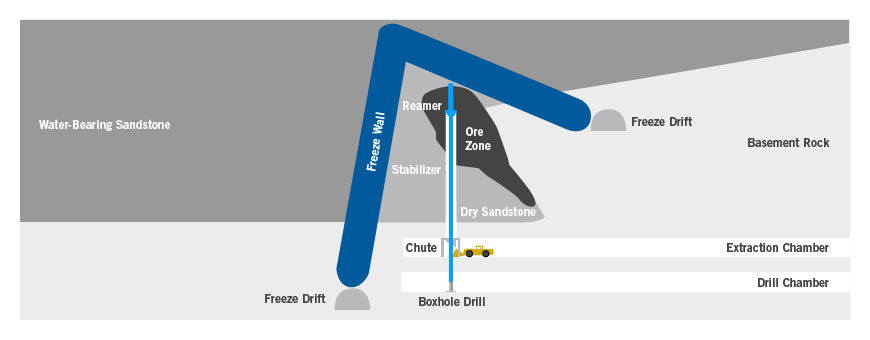
\includegraphics[width=0.9\textwidth]{img/cameco/3.0.1-1MiningMethods-Boxhole.jpg}

Boxhole boring is similar to the \nameref{ssec:raisebore}, but the drilling machine is located below the mineralization, so development is not required above the mineralization. From a drill chamber in waste rock below the ore, we drill a series of overlapping holes up through the ore zone and collect the falling ore from a chute in the extraction chamber. This method is currently being used at a few mines around the world, but had not been used for uranium mining prior to testing at McArthur River.
\subsection*{Blasthole Stoping}


Blasthole stoping involves establishing drill access above the mineralization and extraction access below the mineralization. The area between the upper and lower access levels (the stope) is then drilled off and blasted. The broken rock is collected on the lower level by line-of-sight remote-controlled scoop trams and transported to a grinding circuit. Once a stope is mined out, it is backfilled with concrete to maintain ground stability and allow the next stope in sequence to be mined. This mining method has been used extensively in the mining industry.
\subsection*{Jet Boring}
\label{ssec:jetbore}
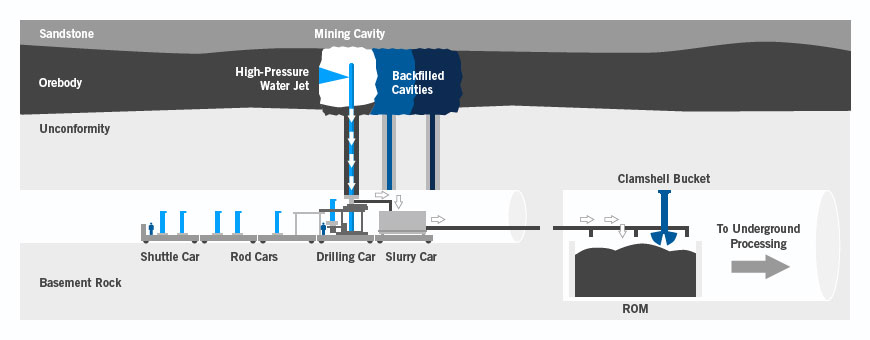
\includegraphics[width=0.9\textwidth]{img/cameco/3.0.1-2MiningMethods-JetBore.jpg}

Jet boring involves freezing the ore and surrounding rock in order to mine safely at Cigar Lake. Brine, chilled to -40C, is piped underground to the deposit. The brine is circulated through large pipes, freezing the surrounding rock in about one year. When ready, a mining machine bores through the frozen rock to create the production tunnel. The jet boring system enters this tunnel and drills a pilot hole through the orebody. Then the jet boring nozzle is inserted in the pilot hole and the system begins boring through the rock using a high-pressure jet of water. Loose ore is flushed down the pilot hole. After a series of processes, ore is pumped to the surface in a slurry form.

\href{https://www.cameco.com/businesses/mining-methods/jet-boring-video}{Watch video}
\subsection*{In Situ recovery}
\label{ssec:insitu}
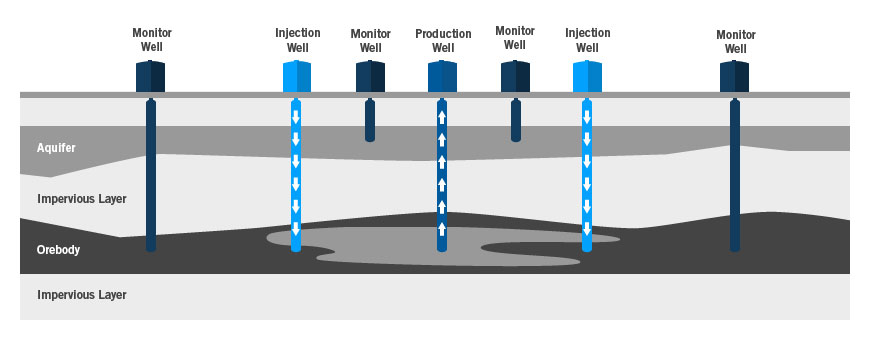
\includegraphics[width=0.9\textwidth]{img/cameco/3.0.1-3MiningMethods-ISR.jpg}

In situ recovery (ISR) methods are applied at our operations in the US and Kazakhstan to extract uranium contained in sandstone aquifers. In situ techniques involve circulation of solutions through ore-bearing formations to dissolve uranium and pump it to the surface for recovery. This approach results in minimal surface disturbance and produces no waste rock or mill tailings.

\href{https://www.cameco.com/businesses/mining-methods/in-situ-recovery-video}{Watch video}
\subsection*{Raisebore Mining}
\label{ssec:raisebore}
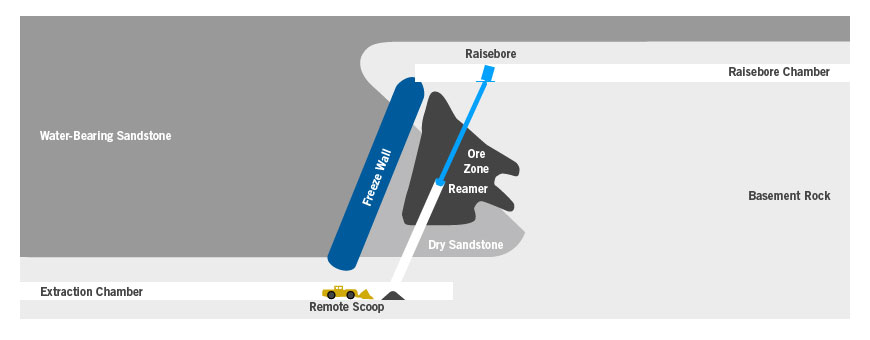
\includegraphics[width=0.9\textwidth]{img/cameco/3.0.1-4MiningMethods-Raisebore.jpg}

Raisebore mining is an innovative non-entry approach that we adapted to meet the unique challenges at McArthur River. From a raisebore chamber in waste rock above the ore, we drill a series of overlapping holes through the ore zone and collect the ore using remote-controlled scoop trams at the bottom of the raises. Once each raisebore hole is complete, we fill it with concrete. We have successfully used the raisebore mining method to extract more than 250 million lbs since we began mining in 1999.
